%% Shared: Wishbone B4 Classic peripheral bus (both variants)
%%%%%%%%%%%%%%%%%%%%%%%%%%%%%%%%%%%%%%%%%%%%%%%%%%%%%%%%%%%%%%%%%%%%%%%%%%%%%
\subsection{Wishbone B4 Classic -- Peripheral Bus}
%%%%%%%%%%%%%%%%%%%%%%%%%%%%%%%%%%%%%%%%%%%%%%%%%%%%%%%%%%%%%%%%%%%%%%%%%%%%%

\subsubsection{Signal Naming Convention}

Wishbone signal names in this design follow the convention shown in
Table~\ref{tab:asBusConcept02}.
The suffix \texttt{\_i} indicates an input, \texttt{\_o} an output,
and \texttt{\_s} an internal wire.
The prefix \texttt{wb\_s\_} is used for slave-side signals and
\texttt{wb\_m\_} for master-side signals.

\begin{table}[H]
\caption{Wishbone Signal Naming}
\label{tab:asBusConcept02}
\centering
\begin{tabularx}{\textwidth}{|l |l |l |l |X|}
  \hline
  Wishbone Name & Slave Port & Master Port & Width & Description \\
  \hline
  \hline
  ADR    & \texttt{wb\_s\_addr\_i} & \texttt{wb\_m\_addr\_o} & 64 & Address bus \\
  \hline
  DAT\_I & \texttt{wb\_s\_dat\_i}  & \texttt{wb\_m\_dat\_i}  & 64 & Data from master to slave (write data) \\
  \hline
  DAT\_O & \texttt{wb\_s\_dat\_o}  & \texttt{wb\_m\_dat\_o}  & 64 & Data from slave to master (read data) \\
  \hline
  WE     & \texttt{wb\_s\_we\_i}   & \texttt{wb\_m\_we\_o}   & 1  & Write enable: 1 = write, 0 = read \\
  \hline
  SEL    & \texttt{wb\_s\_sel\_i}  & \texttt{wb\_m\_sel\_o}  & 8  & Byte select (all bytes must be set) \\
  \hline
  STB    & \texttt{wb\_s\_stb\_i}  & \texttt{wb\_m\_stb\_o}  & 1  & Strobe: valid cycle indicator from master \\
  \hline
  ACK    & \texttt{wb\_s\_ack\_o}  & \texttt{wb\_m\_ack\_i}  & 1  & Acknowledge: normal end of transfer from slave \\
  \hline
  CYC    & \texttt{wb\_s\_cyc\_i}  & \texttt{wb\_m\_cyc\_o}  & 1  & Cycle: bus cycle active (held for complete transfer) \\
  \hline
\end{tabularx}
\end{table}

\subsubsection{Transfer Protocol}

A Wishbone Classic single transfer proceeds as follows:

\begin{enumerate}
  \item The master asserts \texttt{CYC} and \texttt{STB}, presents a valid
    address on \texttt{ADR}, drives \texttt{WE} (1 for write, 0 for read),
    sets \texttt{SEL} to all-ones, and -- for a write -- provides data on
    \texttt{DAT\_O}.
  \item In this implementation the slave responds \emph{combinatorially} in the
    same clock cycle: it drives read data on \texttt{DAT\_O} and asserts
    \texttt{ACK}.
  \item The transaction is complete when both \texttt{STB} and \texttt{ACK}
    are seen high on the rising clock edge.
    The master may then begin a new transfer in the very next cycle.
\end{enumerate}

A transfer is considered valid only when both \texttt{CYC} and \texttt{STB}
are asserted simultaneously and all byte-select bits are set.
If any byte-select bit is clear the BPI treats the access as invalid and
suppresses both the ACK and the write enable to the peripheral.

The timing diagram below illustrates a write followed by a read.

\begin{figure}[H]
\centering
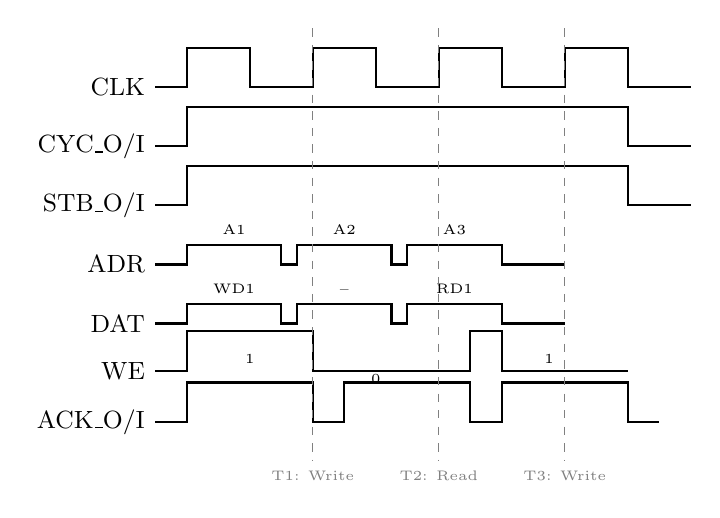
\begin{tikzpicture}[x=0.8cm, y=0.5cm]
  % Clock
  \draw[thick] (0,8) node[left]{\small CLK}
    -- ++(0.5,0) -- ++(0,1) -- ++(1,0) -- ++(0,-1) -- ++(1,0) -- ++(0,1) -- ++(1,0) -- ++(0,-1)
    -- ++(1,0) -- ++(0,1) -- ++(1,0) -- ++(0,-1) -- ++(1,0) -- ++(0,1) -- ++(1,0) -- ++(0,-1) -- ++(1,0);
  % CYC
  \draw[thick] (0,6.5) node[left]{\small CYC\_O/I}
    -- ++(0.5,0) -- ++(0,1) -- ++(7,0) -- ++(0,-1) -- ++(1,0);
  % STB
  \draw[thick] (0,5) node[left]{\small STB\_O/I}
    -- ++(0.5,0) -- ++(0,1) -- ++(7,0) -- ++(0,-1) -- ++(1,0);
  % ADR (two phases)
  \draw[thick] (0,3.5) node[left]{\small ADR}
    -- ++(0.5,0)
    -- ++(0,0.5) -- ++(1.5,0) node[midway,above]{\tiny A1}
    -- ++(0,-0.5) -- ++(0.25,0) -- ++(0,0.5)
    -- ++(1.5,0) node[midway,above]{\tiny A2}
    -- ++(0,-0.5) -- ++(0.25,0) -- ++(0,0.5)
    -- ++(1.5,0) node[midway,above]{\tiny A3}
    -- ++(0,-0.5) -- ++(1,0);
  % DAT (write, then read)
  \draw[thick] (0,2) node[left]{\small DAT}
    -- ++(0.5,0)
    -- ++(0,0.5) -- ++(1.5,0) node[midway,above]{\tiny WD1}
    -- ++(0,-0.5) -- ++(0.25,0) -- ++(0,0.5)
    -- ++(1.5,0) node[midway,above]{\tiny --}
    -- ++(0,-0.5) -- ++(0.25,0) -- ++(0,0.5)
    -- ++(1.5,0) node[midway,above]{\tiny RD1}
    -- ++(0,-0.5) -- ++(1,0);
  % WE
  \draw[thick] (0,0.8) node[left]{\small WE}
    -- ++(0.5,0) -- ++(0,1) -- ++(2,0) -- ++(0,-1) -- ++(2.5,0) -- ++(0,1) -- ++(0.5,0) -- ++(0,-1)  -- ++(2,0);
  \node at (1.5,1.1)  {\tiny 1};
  \node at (3.5,0.6)  {\tiny 0};
  \node at (6.25,1.1) {\tiny 1};
  % ACK
  \draw[thick] (0,-0.5) node[left]{\small ACK\_O/I}
    -- ++(0.5,0) -- ++(0,1) -- ++(2,0) -- ++(0,-1)
    -- ++(0.5,0) -- ++(0,1) -- ++(2,0) -- ++(0,-1)
    -- ++(0.5,0) -- ++(0,1) -- ++(2,0) -- ++(0,-1) -- ++(0.5,0);
  % Labels
  \draw[dashed,gray] (2.5,9.5) -- (2.5,-1.5) node[below]{\tiny T1: Write};
  \draw[dashed,gray] (4.5,9.5) -- (4.5,-1.5) node[below]{\tiny T2: Read};
  \draw[dashed,gray] (6.5,9.5) -- (6.5,-1.5) node[below]{\tiny T3: Write};
\end{tikzpicture}
\caption{Wishbone Classic Single Transfers: Write -- Read -- Write}
\label{fig:asBusTiming01}
\end{figure}

\subsubsection{Byte Select}

The 8-bit \texttt{SEL} signal indicates which byte lanes carry valid data.
Bit\;$n$ of \texttt{SEL} corresponds to byte lane\;$n$ (bits $8n+7\ldots 8n$)
of the 64-bit data bus.
In the current implementation, the master BPI always drives all eight
\texttt{SEL} bits to~1 (full-word transfers only).
The slave BPI checks that all \texttt{SEL} bits are set before asserting
\texttt{ACK} or issuing a write enable to the peripheral kernel.
Sub-word accesses are therefore not supported.

\subsubsection{Reset Behaviour}
\label{subsubsec:wbResetBehaviour}

All Wishbone outputs are driven to their inactive state while the
\textbf{asynchronous}, active-high reset \texttt{rst\_i} is asserted (every
clocked block in this design uses
\texttt{always\_ff\ @(posedge\ clk\_i,\ posedge\ rst\_i)}; there is no
synchronous-reset flip-flop anywhere in the RTL).
For the master BPI this means \texttt{STB\_O} and \texttt{CYC\_O} are held
low; for the slave BPI \texttt{ACK\_O} is held low.
Note that in the current purely combinatorial implementation the reset
is not registered inside the BPI modules; the reset is applied by the
surrounding peripheral logic.

